\documentclass[12pt, letterpaper]{article}

%-------Packages---------
\usepackage{amssymb,amsfonts}
\usepackage{mathptmx}
\usepackage{amsthm}
\usepackage{graphicx}
\usepackage[all,arc]{xy}
\usepackage{enumerate}
\usepackage{bbm}
\usepackage{dsfont}
\usepackage{mathrsfs}
\usepackage{tikz-cd}
\usepackage{setspace}
\usepackage{import}
\usepackage[utf8]{inputenc}
\usepackage{hyperref}
\usepackage{tikz}
\usepackage{float}
\usepackage[dvipsnames]{xcolor}
\usepackage[nocheck]{fancyhdr}
\usepackage[nointegrals]{wasysym}

\usepackage[left=1in,top=1in,right=1in,bottom=1in]{geometry}

\usepackage{mathtools}
\usepackage{setspace}
\usepackage{cleveref}
\usepackage{multicol}
\usepackage{mathpazo}
\usepackage{tcolorbox}
\tcbuselibrary{theorems,skins,breakable}
\usepackage{xparse}

\usepackage{algorithm}
\usepackage[noend]{algpseudocode}

\usepackage{xcolor, ifthen, tcolorbox}
\tcbuselibrary{theorems,skins,breakable}
% Theorem System
% The following environments are provided:
%   New Problem:        \begin{problem} ...
%   New Question Header:   \qh (then followed by subproblems)
%   Subproblem:     \begin{subproblem} ...
%   Problem Proof:  \begin{problemproof} ...
%   Proof:          \\begin{pf}{color} ...
%   Remark:         \rmk (sentence), \rmkb (block)

% Define custom colors
\definecolor{thmscol}{HTML}{F4565B} %For Problems
\definecolor{lemscol}{HTML}{FE844C} %For Lemmes
\definecolor{prpscol}{HTML}{00A7EF} %For proposition
\definecolor{corscol}{HTML}{23DAFF} %For corrolaries
\definecolor{rmkscol}{HTML}{6DEEC5} %For remarks
\definecolor{defscol}{HTML}{18C991} %For definitions
\definecolor{exmscol}{HTML}{7DB800} %For examples
\definecolor{clmscol}{HTML}{165c58} %For claims

%Change between dark(black)/light(white) mode
\newcommand{\colormode}{white}
\ifthenelse{\equal{\colormode}{white}}
      {\newcommand{\TextColor}{black}}
      {\newcommand{\TextColor}{white}}
\newcommand{\pbcolormain}{thmscol!80!\colormode}
\newcommand{\pbcolorsecond}{thmscol!38!\colormode}


% ============================
% Problem Counter
% ============================
\newcounter{subproblemcounter}
\newcounter{problemcounter}

\newcommand{\q}{
    \setcounter{subproblemcounter}{0}%
    \stepcounter{problemcounter} % Increment problem counter
    \color{\TextColor}Problem \arabic{problemcounter}: % Display the problem counter
}

\newcommand{\stepsub}{
    \stepcounter{subproblemcounter}%
    \color{\TextColor}(\alph{subproblemcounter})
}
% ============================
% Problem
% ============================
\newtcolorbox{pb}[1]{
  enhanced,
  frame hidden,
  titlerule=0mm,
  toptitle=1mm,
  bottomtitle=1mm,
  fonttitle=\bfseries\large,
  coltitle=black,
  colbacktitle=\pbcolormain,
  colback=\pbcolorsecond,
  title={\q #1},
  coltext=\TextColor
}

\newtcolorbox{spb}[1]{
  enhanced,
  frame hidden,
  titlerule=0mm,
  toptitle=1mm,
  bottomtitle=1mm,
  fonttitle=\bfseries\large,
  coltitle=black,
  colbacktitle=\pbcolormain,
  colback=\pbcolorsecond,
  title={\stepsub #1},
  coltext=\TextColor,
  attach boxed title to top left={xshift=3mm,yshift=-2mm},
  boxed title style={
    colback=\pbcolormain,
    colframe=\pbcolormain,
  }
}

\newtcolorbox{pbh}[1]{
    enhanced,
    frame hidden,
    titlerule=0mm,
    toptitle=1mm,
    bottomtitle=1mm,
    fonttitle=\bfseries\large,
    coltitle=black,
    colbacktitle=\pbcolormain,
    colback=\pbcolorsecond,
    title={\q #1},
    boxrule=0pt,
    interior hidden,
    attach boxed title to top left={xshift=3mm,yshift=-2mm},
    boxed title style={
        colback=\pbcolormain,
        colframe=\pbcolormain,
    }
}

\newenvironment{problem}[1]{%
  \newpage
  \begin{pb}{#1}
    }{
  \end{pb}
}

\newenvironment{subproblem}[1]{%
  \begin{spb}{#1}
    }{
  \end{spb}
}

\newenvironment{problemproof}{%
    \begin{pf}{\pbcolormain}
        }{
    \end{pf}
}

\newcommand{\qh}[1][]{
    \newpage
    \begin{pbh}{#1}\end{pbh} % Display the problem counter
}

% ============================
% Claim
% ============================

\newtcbtheorem[number within=problemcounter]{claim}{Claim}
{
    enhanced,
    frame hidden,
    titlerule=0mm,
    toptitle=1mm,
    bottomtitle=1mm,
    fonttitle=\bfseries\large,
    coltitle=black,
    colbacktitle=clmscol!50!\colormode,
    colback=clmscol!20!\colormode,
}{clm}

\NewDocumentCommand{\clm}{m+m}{
    \begin{claim*}{#1}{}
        #2
    \end{claim*}
}

\newenvironment{clmpf}{
	{\noindent{\it \textbf{Proof.}}
	\setlength{\parindent}{0pt}
	}
	\tcolorbox[blanker,breakable,left=5mm,parbox=false,
    before upper={\parindent15pt},
    after skip=10pt,
	borderline west={1mm}{0pt}{clmscol!50!\colormode}]
}{
    \textcolor{clmscol!50!\colormode}{\hbox{}\nobreak\hfill$\blacksquare$}
    \endtcolorbox
}

\NewDocumentCommand{\clmp}{m+m+m}{
    \begin{claim*}{#1}{}
        #2
    \end{claim*}

    \begin{clmpf}
        #3
    \end{clmpf}
}


% ============================
% Proof
% ============================

\newenvironment{pf}[1]{%
  \def\pfcolor{#1}% Store the color in a macro
  \noindent{\it \textbf{Proof.}}%
  \tcolorbox[blanker,breakable,left=5mm,parbox=false,%
    before upper={\parindent15pt},%
    after skip=10pt,%
    borderline west={1mm}{0pt}{\pfcolor},%
    coltext=\TextColor
  ]%
  \setlength{\parindent}{0pt}%
}{%
  \textcolor{\pfcolor}{\hbox{}\nobreak\hfill$\blacksquare$}%
  \endtcolorbox%
}

\newtcolorbox{solution}{
  blanker,
  breakable,
  left=5mm,
  parbox=false,%
  before upper={\parindent15pt},%
  after skip=10pt,%
  borderline west={1mm}{0pt}{\pbcolormain},%
  coltext=\TextColor
}


% ============================
% Remark
% ============================


\NewDocumentCommand{\rmk}{+m}{
    {\it \color{rmkscol!100!white}#1}
}

\newenvironment{remark}{
    \par
    \vspace{5pt}
    \begin{minipage}{\textwidth}
        {\par\noindent{\textbf{Remark.}}}
        \tcolorbox[blanker,breakable,left=5mm,
        before skip=10pt,after skip=10pt,
        borderline west={1mm}{0pt}{rmkscol!80!\colormode},
        coltext=\TextColor
        ]
}{
        \endtcolorbox
    \end{minipage}
    \vspace{5pt}
}

\NewDocumentCommand{\rmkb}{+m}{
    \begin{remark}
        #1
    \end{remark}
}


% Define a new command for problems
\renewcommand{\headrule}{\color{\TextColor}\hrulefill}
\newcommand{\C}{\mathbb{C}}
\newcommand{\R}{\mathbb{R}}
\newcommand{\Q}{\mathbb{Q}}
\newcommand{\Z}{\mathbb{Z}}
\newcommand{\N}{\mathbb{N}}
\renewcommand{\P}{\mathsf{P}}
\newcommand{\NP}{\mathsf{NP}}
\newcommand{\F}{\mathbb{F}}
\newcommand{\T}{\mathcal{T}}
\newcommand{\contr}{\Rightarrow \Leftarrow}
\newcommand{\s}{\(\,\)}
\renewcommand{\t}[1]{\text{#1}}
\newcommand{\ang}[1]{\left\langle #1 \right\rangle}
\newcommand{\coker}{\mathrm{coker}}

% Meta data
\setstretch{1.2}

\begin{document}
\color{\TextColor}
\pagecolor{\colormode}
\setlength{\parindent}{0pt}
\pagestyle{fancy}
\fancyhf{}
\fancyhead[LOE]{\color{\TextColor}\slshape{\textbf{Vincent Ferrara}}}
\fancyhead[ROE]{\color{\TextColor}\thepage}

\qh[Self assessment.]
\begin{solution}
    In question 6 part (b), I believe my solution is an improvement over the provided one. Their function \( g \) is unnecessarily complicated by treating the case \( k > |V| \) separately. Notice that if \( k > |V| \), then \((G, K_k)\) cannot be a subgraph isomorphism because \(K_k\) has more vertices than \(G\). By simply defining \( g(G, k) = (G, K_k) \), the logic is simplified while still capturing the necessary conditions. This streamlined approach demonstrates that my solution is both more concise and effective.
\end{solution}

\qh[True, false, or unknown.]

\begin{subproblem}{}
    If $\P \neq \NP$ and $L$ is $\NP$-complete, then $L \notin \P$.
\end{subproblem}
\begin{problemproof}
    Assume $\P \neq \NP$. Let $L$ be $\NP$-complete.

    Assume for contradiction that $L \in \P$.

    Since $L$ is $\NP$-complete. This means that $L \in \NP$ and every $\NP$ problem reduces to $L$.

    Thus, let $A \in \NP$. Thus, $A \leq_p L$. Since $L \in P$, by proven in class this implies that $A \in \P$.

    Therefore, $\NP \subset P \implies \P = \NP$ which is a contradiction. Thus, $L \notin P$.
\end{problemproof}

\begin{subproblem}{}
    If $L\in\NP$, then $L \in \P$.
\end{subproblem}
\begin{problemproof}
    This is unknown, since if it were true then this would imply $\NP \subset \P \implies \NP = \P$. If it were false then we know there is a $L \in \NP$ s.t. $L \notin \P \implies \P \subsetneq \NP \implies \P \neq \NP$. Both of these results are unknown.
\end{problemproof}
\newcommand{\SAT}{\textsc{SAT}}
\begin{subproblem}{}
    Let $V$ be an efficient verifier for some language $L \in \NP$. Let $f$ be the Cook-Levin mapping reduction from $L$ to $\SAT$. The function $f(x)$ selects a certificate $c$, runs $V(x,c)$, and construct a Boolean formula $\phi$ from its computational tableau. 
\end{subproblem}
\begin{problemproof}
    False.

The Cook-Levin reduction does not work by “selecting” a certificate \( c \) and running \( V(x,c) \). Instead, it constructs a Boolean formula \(\phi\) that is satisfiable if and only if there exists some certificate \( c \) that would make \( V(x,c) \) accept.
\end{problemproof}
\newcommand{\TSP}{\textsc{TSP}}
\newcommand{\HC}{\textsc{HAMCYCLE}}
\newcommand{\ptimemap}{\leq_p}
\newcommand{\set}[1]{\{#1\}}
\qh[$\Upsilon$'s alternative reductions.]
\begin{subproblem}{}
      \begin{minipage}{0.9\textwidth}
      \begin{center}
    \begin{algorithm}[H]
      \begin{algorithmic}[1]
      \Require{An unweighted graph $G$}
      \Ensure{A weighted graph $G'$ and nonnegative integer $k$}
        \Function{$f$}{$G=(V,E)$}
        \State $V' \gets V$
        \State Initialize $G'$ to be a complete graph on $V'$ and initialize all weights to $\infty$ in $E'$
        \State Initialize $C$ to be an empty sequence of vertices
        \For{each permutation $\Pi = (v_1, v_2, \ldots, v_n)$ of $V$}
            \If {$(v_i, v_{i+1}) \in E$ for all $i = 1, \ldots, n-1$} 
                \State $C \gets \Pi$
                \State \textbf{break}
            \EndIf
        \EndFor
        \For {each adjacent pair $(v_i, v_{i+1})$ in $C$}
            \State Set the weight of $(v_i, v_{i+1})$ to be 1 in $E'$
        \EndFor
        \State \Return $(G'=(V', E'), k=|V|)$
        \EndFunction
      \end{algorithmic}
    \end{algorithm}
    \end{center}
    \end{minipage}
\end{subproblem}
\begin{problemproof}
    The reduction fails because it iterates over every permutation of the vertices, which takes factorial time. This factorial time complexity means the reduction does not run in polynomial time, so it does not serve as a valid polynomial-time mapping reduction.
\end{problemproof}

\begin{subproblem}{}
    \begin{itemize}
        \item For each variable $x \in \phi$, create a variable gadget
         consisting of two vertices, respectively labeled by the literals $x$ and $\overline x$, with \emph{no edges between them}. 
         \item For each clause $(\ell_i \lor \ell_j \lor \ell_k)$ in $\phi$, create a clause gadget of three vertices, respectively labeled by these literals, with an edge between each pair of these vertices (i.e., a triangle).
         \item For each vertex of each clause gadget, create an edge between that vertex and the (unique) variable-gadget vertex having the same label. 
         \item Finally, set $k = n+2m$, where $n$, $m$ are respectively the number of variables and clauses in $\phi$. 
    \end{itemize}
\end{subproblem}
\begin{problemproof}
    The mistake is that by removing the edge between the two literal vertices in each variable gadget, you lose the “forcing” mechanism that guarantees one of the two must be chosen in a minimum vertex cover. In the standard reduction, the edge between \(x\) and \(\neg x\) forces the vertex cover to include at least one vertex from each variable gadget—ensuring that exactly one literal is “selected” per variable (since including both would exceed the budget). Without that edge, the reduction no longer forces a choice, and a vertex cover of size \(n + 2m\) might be obtained by not “selecting” any literal for some variables. This breaks the correspondence between vertex covers and satisfying assignments for the \textsc{3SAT} instance, rendering the reduction incorrect.
\end{problemproof}
\newcommand{\Coloring}
{\textsc{Coloring}}
\newcommand{\Schedule}{\textsc{Scheduling}}
\begin{problem}{Scheduling exams with flying colors.}
    \vspace{-20pt}
    \[\Schedule = \set{(S, C, k): \exists f: C \rightarrow \{1 \ldots k\} \text{ s.t } f(C_i) = f(C_j) \implies C_i \cap C_j = \emptyset}\]
\end{problem}

\begin{subproblem}{}
    Determine if each of the following is an instance of $\Coloring$. If $(G,k) \in \Coloring$, give a coloring of the graph. Otherwise, briefly explain why it's not possible.

    \begin{enumerate}[(i)]
        \item $G = $
            \begin{minipage}{0.3\linewidth}
            \centering
    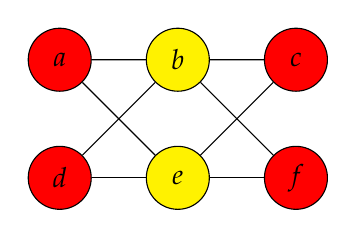
\begin{tikzpicture}[scale=1.5, every node/.style={draw, circle, minimum size=0.8cm, inner sep=0pt}]
        % Define the nodes
        \node[fill=red] (A) at (0,1) {$a$};
        \node[fill=yellow] (B) at (1,1) {$b$};
        \node[fill=red] (C) at (2,1) {$c$};
        \node[fill=red] (D) at (0,0) {$d$};
        \node[fill=yellow] (E) at (1,0) {$e$};
        \node[fill=red] (F) at (2,0) {$f$};
    
        \begin{scope}[every node/.style={auto, draw=none}]
        \draw (A) -- (B);
        \draw (A) -- (E);
        \draw (B) -- (C);
        \draw (B) -- (D);
        \draw (B) -- (F);
        \draw (C) -- (E);
        \draw (D) -- (E);
        \draw (E) -- (F);
        \end{scope}
    \end{tikzpicture}
            \end{minipage}
            , $k = 3$

            \begin{solution} \end{solution}
            
            \item $G = $
            \begin{minipage}{0.3\linewidth}
            \centering
    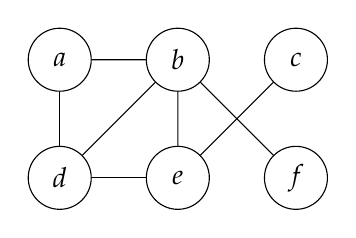
\begin{tikzpicture}[scale=1.5, every node/.style={draw, circle, minimum size=0.8cm, inner sep=0pt}]
        % Define the nodes
        \node (A) at (0,1) {$a$};
        \node (B) at (1,1) {$b$};
        \node (C) at (2,1) {$c$};
        \node (D) at (0,0) {$d$};
        \node (E) at (1,0) {$e$};
        \node (F) at (2,0) {$f$};
    
        \begin{scope}[every node/.style={auto, draw=none}]
        \draw (A) -- (B);
        \draw (A) -- (D);
        \draw (B) -- (D);
        \draw (B) -- (E);
        \draw (B) -- (F);
        \draw (C) -- (E);
        \draw (D) -- (E);
        \end{scope}
    
    \end{tikzpicture}
    \end{minipage}
    , $k = 2$
\end{enumerate}
\end{subproblem}
\begin{problemproof}
    This configuration is not possible for case (ii) because if we assign one color to (a), then both (b) and (d) must use the only remaining color. However, since (b) and (d) are adjacent, they cannot share the same color, leaving us without a valid coloring option.
\end{problemproof}

\begin{subproblem}{}
    Show that $\Coloring \ptimemap \Schedule$. Since $\Coloring$ is $\NP$-hard, $\Schedule$ is $\NP$-hard.
\end{subproblem}
\begin{problemproof}
    Define: $g:\Sigma^* \to \Sigma*$ s.t. $g(G=(V,E),k)=(S,C,k)$. Let $V=\{v_1,\dots,v_n\}$

    We will define $S=E$, and $C=\{C_1,\dots,C_n\}$ where each $C_i=\{e \in E \mid e=(v_i,v) \t{ for some } v \in V\}$

    Runtime:

    This will take $O(|E|)$ to copy $E$ into $S$. Then it will take $O(|V|+|E|)$ to construct $C$ since we first make a size $|V|$ list then add $2|E|$ edges in total to the $C_i$'s. Thus, the whole function takes $O(|V|+|E|)$ which is polynomial with respect to $|G|$.

    Correctness:

    If $G$ is $k$-colorable then suppose there is a valid coloring $c: V \to \{1,\dots,k\}$. This functions just colors the vertices. Then consider $g(G,k)=(S,C,k)$.

    Define: $f : C \to \{1,\dots,k\}$ s.t. $f(C_i)=c(v_i)$.

    If $f(C_i)=f(C_j)$ for $i \neq j$ then this implies that $c(v_i) = c(v_j)$. This implies that $v_i$ and $v_j$ cannot be adjacent to each other thus $C_i \cap C_j =\emptyset$ since if it was not empty this would imply that either $(v_i,v_j) \in C_i \cap C_j$, but this is not possible since they are not adjacent.

    If $g(G,k)=(S,C,k)$ is a valid scheduling then this implies there is a function 
    
    $f : C \to \{1,\dots,k\}$ s.t. $f(C_i)=f(C_j) \implies C_i \cap C_j =\emptyset$.

    Define: $c : V \to \{1,\dots,k\}$ s.t. $c(v_i)=f(C_i)$.

    Consider $v_i,v_j$ s.t. $(v_i,v_j) \in E$, by definition of each $C_i$ and $C_j$ this would imply that $(v_i,v_j) \in C_i \cap C_j$. Thus, $f(C_i) \neq f(C_j) \implies c(v_i) \neq c(v_j)$. This implies that $c$ is a valid coloring since for each adjacent vertices they are a different colors.

    Thus, $\Coloring \ptimemap \Schedule$
\end{problemproof}
\newcommand{\Clique}{\textsc{Clique}}
\newcommand{\Recipe}{\textsc{Bussin-Recipe}}
\begin{problem}{This recipe is bussin but $\NP$-hard.}
    \[
        \Recipe =
    \]
    \[\set{(D, m, p) : D \in \set{0 \ldots 10}^{n \times n} \text{, } \exists S \subseteq \{1 \ldots n\} \text{ s.t } |S| \geq m \text{ and } \sum_{i,j \in S} D_{ij} \leq p}\]
    We assume for simplicity that $D_{ij} = D_{ji}$ and $D_{ii} = 0$ for all $i,j = 1, \ldots n$. 
    
Show that \Recipe$\;$is $\NP$-hard.
\end{problem}
\begin{problemproof}
    WTS: $\Clique \leq_p \Recipe$

    Define: $g:\Sigma^* \to \Sigma*$ s.t. $g(G=(V,E),k)=(D,k,0)$. Let $V=\{v_1,\dots,v_n\}$

    We will let $D_{ii}=0$, and $D_{ij}=D_{ji}=0$ if $(v_i,v_j) \in E$ and $D_{ij}=D_{ji}=10$ if $(v_i,v_j) \notin E$.

    Runtime:

    It will take $O(|V|^2)$ to make $D$ since $|D|=|V|^2$, and the rest are $O(1)$ operations, assuming $E$ is made with a set data structure. Thus, the runtime is $O(|V|^2)$ which is polynomial with respect to $|G|$.

    Correctness:

    If $(G,k) \in \Clique$ then we know we have a subset $C$ of $V$ s.t. for all $v,u \in C$ that $(v,u) \in E$, and $|C| \geq k$.

    Therefore, we know that $g(G,k)=(D,k,0)$. Since we know that for all pairs of vertices in $C$ that they are connected. This implies that $D_{ij}=0$ for all $v_i,v_j \in C$. Since $C$ is at least size $k$ we know we can just pick $S=\{i_1,\dots,i_k\}$ s.t. $v_{i_j} \in C$.

    Therefore, since each $D_{ij}=0$ we know that $\sum_{i,j \in S} D_ij = 0 =p$. Thus, $(D,k,0) \in \Recipe$

    If $g(G,k)=(D,k,0) \in \Recipe$ this implies that there is a subset $S=\{i_1,\dots,i_r\}$ s.t. $|S| \geq k$. By definition of $D$ since we know that each $D_{ij}=0$ for $i,j \in S$. This implies that $(v_i,v_j) \in E$. Therefore, since we know that all pairs in $S$ have $D_{ij}=0$. This implies that all pairs of vertices $v_i,v_j$ are connected in $G$. This is exactly the definition of a clique, and since we have at least size $|S|\geq k$. Thus, $(G,k) \in \Clique$.

    Therefore, $\Clique \leq_p \Recipe$ which implies $\Recipe$ is $\NP$-Hard
\end{problemproof}
\newcommand{\SSUM}{\textsc{SUBSET-SUM}}
\begin{problem}{Subset sum.}
    \vspace{-20pt}
    \[ \SSUM = \set{(A, s) : A \text{ is a multiset of integers $\geq 0$, and } \exists\; I \subseteq A \text{ s.t } \sum_{a \in I} a = s}.
  \]
  The reduction is as follows.
  As input it is given a 3CNF formula~$\phi$ with~$n$ variables $x_1, \ldots, x_n$ and~$m$ clauses $c_1, \ldots, c_m$.
  (Recall that each clause is the OR of exactly three literals, where a literal is either some variable~$x_{i}$ or its negation $\overline{x_{i}}$.)

  The reduction constructs a collection of numbers as follows:

  \begin{enumerate}
  \item For each clause $c_j$, it constructs integers $a_j=b_j$, which are $m + n$ decimal digits long (counting any leading zeros), whose $j$th digits are~1, and whose other digits are~0.
  \item For each variable $x_i$, it constructs integers $t_i$ and $f_i$, each $m + n$ decimal digits long, where:
    \begin{enumerate}
    \item The $(m + i)$th digits of both $t_i$ and $f_i$ are 1.
    \item The $j$th digit of $t_i$ is 1 if literal $x_i$ appears
      in clause $c_j$.
    \item The $j$th digit of $f_i$ is 1 if literal $\overline{x_i}$
      appears in clause $c_j$.
    \item All other digits of $t_i$ and $f_i$ are 0.
    \end{enumerate}
  \item It constructs a target sum~$s$ that has $m + n$ decimal digits, where the first~$m$ digits are~\textbf{[TODO: Part a]} and the last~$n$ digits are~\textbf{[TODO: Part a]}. 
  \end{enumerate}
  The reduction outputs $(A,s)$, where $A$ is the set of all the numbers $a_{j}$, $b_{j}$, $t_{i}$, and~$f_{i}$.
\end{problem}

\begin{subproblem}{}
    Give the complete step 3 from the description above. You do not need to justify your answer.
\end{subproblem}
\begin{solution}
    The first $m$ digits are $3$, and the last $n$ digits are $1$.
\end{solution}

\begin{subproblem}{}
    The $\SSUM$ instance for the given formula~$\phi$ is therefore
  \[ A=\set{10000,10000,1000,1000,10100,1100,1010,10010,10001,1001},s=?
  \]
    Based on your answer in Part a, determine $s$ in the example given above. Then, show that $(A,s)$ is an instance of $\SSUM$ by giving a subset of $A$ that sums to $s$.
\end{subproblem}
\begin{solution}
    $s=33111$

    \noindent Consider $\{a_1,a_2,b_2t_1,t_2,t_3\}$. $10000+01000+01000+10100+01010+10001=33111$. Thus, $(A,s) \in \SSUM$.
\end{solution}
\newcommand{\TSAT}{\textsc{3SAT}}
\begin{subproblem}{}
    Using the reduction described above, construct the $\SSUM$ instance corresponding to the $\TSAT$ instance $\phi' = (x_1 \vee x_1 \vee x_1)\wedge (\overline{x_1}\vee \overline{x_1}\vee \overline{x_1})$.
    (Note that~$\phi'$ is not satisfiable.)
    Also state whether the output instance is in the language $\SSUM$.
\end{subproblem}
\begin{problemproof}
    $A=\{a_1,a_2,b_1,b_2,t_1,f_1\}=\{100,10,100,10,101,11\}$, $s=331$.

    $(A,s) \notin \SSUM$ since look at the last digit of $s$. It is one this implies that we must pick either $t_1$ or $f_1$ but not both.

    If we pick $t_1$ then our current sum is $101$. Thus, we need $230$ more. However, this is not possible since the sum of $a_1+a_2+b_1+b_2=220$, which is not enough to get to $s$.
\end{problemproof}

\begin{subproblem}{}
    Show that
    \[ \phi \in \TSAT \implies f(\phi) = (A,s) \in \SSUM.\]
\end{subproblem}
\begin{problemproof}
    Assume $\phi \in \TSAT$. Let $\phi$ have $n$ variables, and $k$ clauses. This implies we have a function $\tau :\{x_1,\dots,x_n\} \to \{True, False\}$ that satisfies $\phi$.

    Consider $f(\phi)=(A,s)$.

    $A=\{a_1,a_2,\dots,a_k,b_1,\dots,b_k,t_1,f_1,\dots,t_n,f_n\}$.

    Consider the sum $S=\displaystyle\sum_{i = 1}^n c_i$ s.t. $c_i=t_i$ if $\tau(x_i)=True$ and $c_i=f_i$ otherwise. Format it to be a $k+n$ long digit with leading zeros if need be.

    Since we only picked either $t_i$ or $f_i$ but not both this means that the $k+i$ spot is a $1$, so for all $1 \leq i \leq n$ we have $k+i$th spot is a one in $S$. Thus, we know that $s$ and $S$ are the same for this part.

    Now consider the first $k$ digits. Assume for contradiction that in the sum $S$ spot $j$ of the first $k$ digits is zero. This would mean that clause for $j$, $\tau$ would not pick any $x_i, \overline{x_i}$ in the clause s.t. it was true. This is a contradiction of $\phi$ being satisfiable.

    Therefore, we know that all of the first $k$ digits are at least $1$. The digits can also not be greater than $3$. Since we know by definition that for the $j$th spot that there is only a max of three $t_i$'s $f_i$'s that have a one in that spot. Since if not this would imply there are more than three literals in a clause which is not possible.

    Thus, we know that the digit is either $1,2,3$. If it is one then add $a_i,b_i$ to it. If it is two then add $a_j$ to it.

    Thus, we we add each $a_i,b_i$ as neccessary we get that all the first $k$ digits will now be $3$ in our sum. Thus, we get the sum we want since the first $k$ digits are 3, and the last $n$ are 1.

    Thus, $(A,s) \in \SSUM$
\end{problemproof}

\begin{subproblem}{}
    Show that
    \[ \phi \in \TSAT \impliedby f(\phi) = (A,s) \in \SSUM.\]
\end{subproblem}
\begin{problemproof}
    Assume $f(\phi)=(A,s) \in \SSUM$. Let $\tau$ have $k$ clauses, and $n$ variables.

    Thus, we know there is a multiset $I \subset A$ s.t. $\sum_{a \in I} a = s$.

    Consider the last $n$ digits of $s$. These are all ones, so consider spot $k+i$. By definition of $f$, we know that only $t_i,f_i$ have a one in the $k+i$th place. This implies that either $t_i$, or $f_i \in I$ but not both for all $i$.

    Therefore, define $\tau : \{x_1,\dots,x_n\} \to \{True, False\}$ s.t. $\tau(x_i)=True$ if $t_i \in I$ otherwise $False$.

    Now consider the first $k$ digits in $s$. Consider the $j$th one. The $j$th spot is 3. Assume for contradiction that for all $f_a,t_b$ s.t. they have a one in the $j$th spot that they are not in $I$. This is not possible since the sum must be a $3$ in that spot, but there are only two other numbers if we exclude the $f_a,t_b$. These are $a_j,b_j$. Thus, we know that at least one $f_a,t_b \in I$ s.t. they have a one in the $j$th spot.

    Now suppose for contradiction that $\tau$ does not satisfy $\phi$. This means that for some clause $c_j$ is not satisfied. Then by definition of $\tau$ this would imply that no $t_a,f_b$ would contribute to a positive value in the $j$th digit, but as shown above this is not possible. Therefore, $\tau$ does satisfy $\phi$. Thus, $\phi \in \TSAT$
\end{problemproof}

\qh[Cook-Levin windows.]
\begin{subproblem}{}
    Specify \emph{all} the valid $2 \times 3$ window contents that could appear in two adjacent rows of the tableau, if those rows represent the verifier TM taking the following transition:
  \begin{center}
    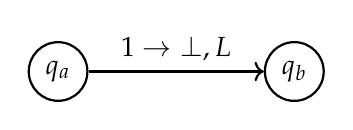
\begin{tikzpicture}
      % Draw circles
      \node[circle,draw,thick] (qa) at (0,0) {$q_a$};
      \node[circle,draw,thick] (qb) at (3,0) {$q_b$};
      
      % Connect circles with arrow
      \draw[->, thick] (qa) -- (qb) node[midway, above] {$1\to \bot,L$};
    \end{tikzpicture}
  \end{center}
\end{subproblem}
\begin{solution}
    \[
    \begin{array}{|c|c|c|}
      \hline
      s_1 & s_2 & s_3 \\
      \hline
      s_1 & s_2 & s_3 \\
      \hline
    \end{array}
    \quad
    \begin{array}{|c|c|c|}
        \hline
        q_a & 1 & s_3 \\
        \hline
        s_1 & \bot & s_3 \\
        \hline
    \end{array}
    \quad
    \begin{array}{|c|c|c|}
          \hline
          s_1 & q_a & 1 \\
          \hline
          q_b & s_1 & \bot \\
          \hline
    \end{array}
    \quad
    \begin{array}{|c|c|c|}
        \hline
        s_1 & s_2 & q_a \\
        \hline
        s_1 & q_b & s_2 \\
        \hline
    \end{array}
    \quad
    \begin{array}{|c|c|c|}
        \hline
        s_1 & s_2 & s_3 \\
        \hline
        s_1 & s_2 & q_b \\
        \hline
    \end{array}
  \]
  $s_1,s_2,s_3 \in \{0,1,\bot\}$
\end{solution}

\begin{subproblem}{}
    Give an example by first defining one or more Turing machine transitions, then providing two adjacent rows where each $2 \times 2$ window is valid, but the transition is incorrect. 
\end{subproblem}
\begin{problemproof}
    Consider \begin{center}
        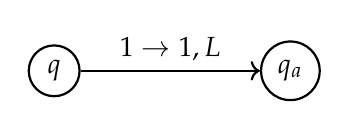
\begin{tikzpicture}
            % Draw circles
            \node[circle,draw,thick] (qa) at (0,0) {$q$};
            \node[circle,draw,thick] (qb) at (3,0) {$q_a$};
            
            % Connect circles with arrow
            \draw[->, thick] (qa) -- (qb) node[midway, above] {$1\to 1,L$};
          \end{tikzpicture}
    \end{center}
    \begin{center}
        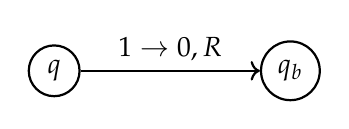
\begin{tikzpicture}
            % Draw circles
            \node[circle,draw,thick] (qa) at (0,0) {$q$};
            \node[circle,draw,thick] (qb) at (3,0) {$q_b$};
            
            % Connect circles with arrow
            \draw[->, thick] (qa) -- (qb) node[midway, above] {$1\to 0,R$};
          \end{tikzpicture}
    \end{center}

    Look at the tape's

    Row $i$: \hspace{17pt} $\dots 1 q 1 1 \dots$

    Row $i+1$: $\dots 1 1 1 1 \dots$

    All valid 2x2 Windows:
    \[\begin{array}{|c|c|}
        \hline
        1 & q \\
        \hline
        1 & 0 \\
        \hline
    \end{array}
    \quad
    \begin{array}{|c|c|}
        \hline
        q & 1 \\
        \hline
        0 & 1 \\
        \hline
    \end{array}
    \quad
    \begin{array}{|c|c|}
        \hline
        1 & 1 \\
        \hline
        1 & 1 \\
        \hline
    \end{array}\]

    However, this is not a valid Turing machine since we get rid of the head.
\end{problemproof}

\begin{subproblem}{}
    Towards proving the Cook-Levin Theorem in lecture, we outlined a proof of the following statement: 
    \begin{quote}
      Let language $L \in \NP$ be arbitrary, and fix an efficient verifier $\textsc{VerifyL}$ for~$L$.
      Given any instance $x$ of $L$, in polynomial time we can construct an instance $\phi$ of $\SAT$ such that $\phi$ is satisfiable \emph{if and only if} there \emph{exists} a $c$ such that the tableau of $\textsc{VerifyL}(x,c)$ has $q_\text{accept}$ in it.
    \end{quote}
    Briefly explain why proving this statement proves that SAT is $\NP$-hard.
\end{subproblem}
\begin{problemproof}
    The statement shows that for any language \(L\) in \(\NP\) and any instance \(x\) of \(L\), we can transform \(x\) into a Boolean formula \(\phi\) such that

\[
x \in L \iff \exists\t{$c$ s.t. \textsc{VerifyL}}(x,c) \t{ accepts.} \iff \phi \in \SAT\,.
\]

This transformation is computable in polynomial time. Since \(L\) was arbitrary, this means that every problem in \(\NP\) can be reduced in polynomial time to SAT. By definition, this is exactly what it means for SAT to be \(\NP\)-hard.
\end{problemproof}

\newcommand{\PSPACE}{\mathsf{PSPACE}}
\newcommand{\EXPTIME}{\mathsf{EXPTIME}}
\newcommand{\TQBF}{\textsc{TQBF}}

\qh[$\PSPACE$ and $\TQBF$]
\begin{subproblem}{}
    Determine the base case when $t = 1$.
\end{subproblem}
\begin{problemproof}
    When \(t=1\), the base case \(\phi_{c_1,c_2,1}\) states that machine \(M\) can go from configuration \(c_1\) to configuration \(c_2\) in at most one step. This can be captured by a Boolean condition that checks whether (1) \(c_1\) is already an accepting configuration and thus equals \(c_2\), or (2) \(c_2\) is exactly the successor configuration obtained by applying one step of \(M\)'s transition function on \(c_1\). In the second case, we verify that the tape contents, head position, and internal state of \(c_2\) match the outcome of executing a single transition from \(c_1\).
\end{problemproof}

\begin{subproblem}{}
    Surprisingly, assuming the base case is correct, $\Upsilon$'s reduction is actually correct. However, it is not efficient. Briefly explain why.
\end{subproblem}
\begin{problemproof}
    Because the naive recursive construction “unrolls” over all possible times up to \(T\), and \(T\) can be as large as \(2^{p(n)}\) for some polynomial \(p\), the resulting formula can grow to exponential (or worse) size in \(n\). In other words, writing down \(\phi_{c_\text{start}, c_\text{accept}, T}\) explicitly requires \(\Omega(T)\) steps just to construct all subformulas, which is not polynomial-time in the length of the input.
\end{problemproof}

\begin{subproblem}{}
    Explain how you would fix $\Upsilon$'s reduction so that it is efficient. Briefly justify its correctness and determine the size of $\phi_{c_\text{start}, c_\text{accept}, T}$. 
\end{subproblem}
\begin{problemproof}
    A more efficient approach modifies \(\Upsilon\)’s naive construction by introducing a \emph{divide-and-conquer} style encoding of the “reachability within \(T\) steps” relation and using \(\forall\)-quantified variables to avoid explicitly writing out subformulas for every time index. Specifically, instead of unrolling the statement “\(M\) goes from \(c_1\) to \(c_2\) in \(\le t\) steps” for each time from 1 to \(T\), we introduce a middle configuration \(c_m\) and say “there \emph{exists} \(c_m\) such that \(M\) goes from \(c_1\) to \(c_m\) in \(\le t/2\) steps and from \(c_m\) to \(c_2\) in \(\le t/2\) steps.” Critically, rather than duplicating the subformulas for every \((c_1,c_2,t)\), we quantify over all configurations and time values universally. In other words, we create a single “template” subformula \(\phi_{c_1,c_2,t}\) and assert it holds \emph{for all} valid triples \((c_1,c_2,t)\). This collapses the exponential blow-up that arises from naive recursion because we only write one copy of the subformula per “level” of the recursion, and we reuse it for all relevant triples by binding them with universal quantifiers.  

This construction is both correct and efficient. It remains correct because halving the time repeatedly captures exactly all ways to reach \(c_2\) from \(c_1\) in up to \(T\) steps: a path of length \(T\) always decomposes into two paths of length \(T/2\). Moreover, the universal quantification over \((c_1,c_2,t)\) ensures that the subformula applies to \emph{every} portion of the computation without needing to explicitly rewrite it each time. The size of the resulting QBF is polynomial in \(\lvert w\rvert\) because: (1) each configuration’s description is polynomial in \(\lvert w\rvert\); (2) the depth of the recursion is \(O(\log T)\), and \(T\) itself is at most \(2^{p(\lvert w\rvert)}\), so \(\log T\) is polynomial in \(\lvert w\rvert\); and (3) we do not replicate subformulas for every single time step but instead reuse them via universal quantifiers. As a result, the overall formula \(\phi_{c_\text{start}, c_\text{accept}, T}\) can be constructed in time (and size) polynomial in \(\lvert w\rvert\), making it a valid polynomial-time reduction.
\end{problemproof}
\end{document}